\documentclass[14pt,fleqn]{extarticle}
\RequirePackage{prepwell-eng}

\previewoff

\begin{document} 
\begin{skill}
    \begin{narrow}
         \textcolor{blue}{Section formula}
         
         Finding the coordinates of the point that divides a \underline{line segment} 
         in the ratio $m:n$
    \end{narrow}
    
    \reason 
    
    The figure below shows a \underline{line segment $AB$} that is divided at $P$ in the ratio $m:n$ \newline 
    
    \begin{center}
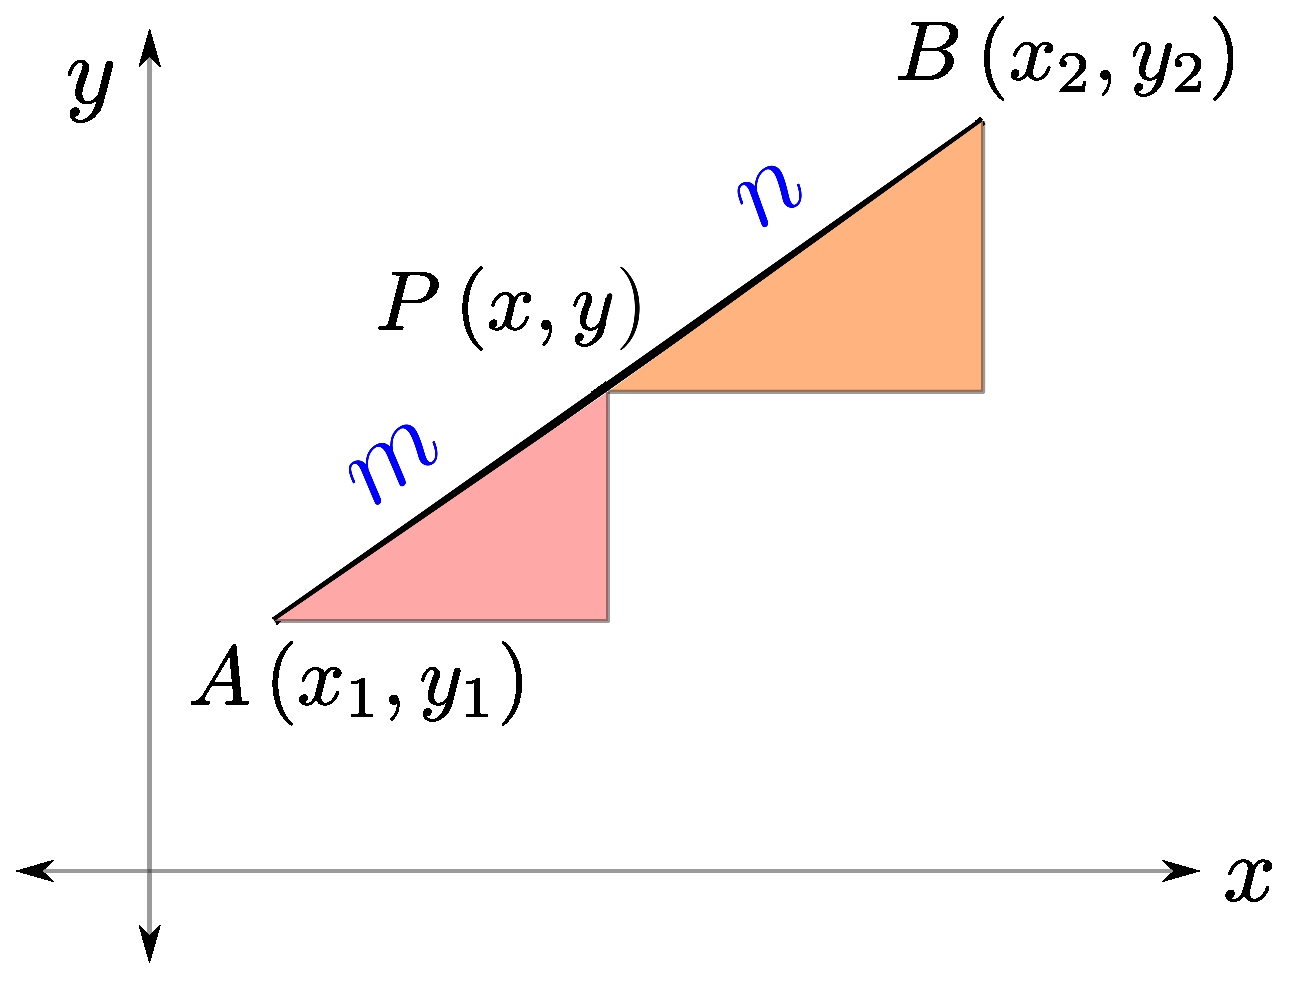
\includegraphics[scale=1.65]{136-A.eps}
\end{center}
    
    From the figure, we can see that 
    \begin{align}
	x &= x_1 + \left(\frac{m}{m+n} \right)\cdot \left(x_2 - x_1 \right) \\
	\implies x &= \frac{mx_2 + nx_1}{m+n}
\end{align}
Similarly, 
\begin{align}
	y &= y_1 + \left(\frac{m}{m+n} \right)\cdot \left(y_2 - y_1 \right) \\
	\implies y &= \frac{my_2 + ny_1}{m+n} \\
	\therefore P &= \left(\frac{mx_2 + nx_1}{m+n}, \frac{my_2 + ny_1}{m+n} \right)
\end{align}

\textbf{Mid-point Formula} \newline 
If $m:n = 1:1$, then $P$ is the mid-point of $AB$. And therefore 
\[ \qquad \underbrace{P = \left(\frac{x_1 + x_2}{2}, \frac{y_1+y_2}{2} \right)}_{m : n = 1:1}\]
    
\end{skill}
\end{document} 